\documentclass[12pt, a4paper]{article}

\usepackage{array}
\usepackage[portuguese]{babel}
\usepackage{chngpage}
\usepackage{float}
\usepackage[a4paper, margin=2cm]{geometry}
\usepackage{graphicx}
\usepackage{hyperref}
\usepackage{setspace}
\usepackage{xcolor}

\title{\Huge \textbf{Computação Gráfica \\ \Large Trabalho Prático -- Fase I}}
\date{2 de março 2025}
\author{Grupo \textbf{\color{red} TODO}}

\begin{document}

\begin{center}
    
\includegraphics[width=0.25\textwidth]{res/cover/EE-C.eps}
\end{center}

\chardef\_=`_
\onehalfspacing
\setlength{\parskip}{\baselineskip}
\setlength{\parindent}{0pt}
\def\arraystretch{1.5}

{\let\newpage\relax\maketitle}
\maketitle
\thispagestyle{empty}

\vspace*{\fill}

\begin{adjustwidth}{-2cm}{-2cm} % These values only need to be large enough to center the table
    \begin{center}
        \begin{tabular}{>{\centering}p{0.25\textwidth}
                        >{\centering}p{0.25\textwidth}
                        >{\centering}p{0.25\textwidth}
                        >{\centering\arraybackslash}p{0.25\textwidth}}
            
\includegraphics[width=3.5cm]{res/cover/A104437.png} &
            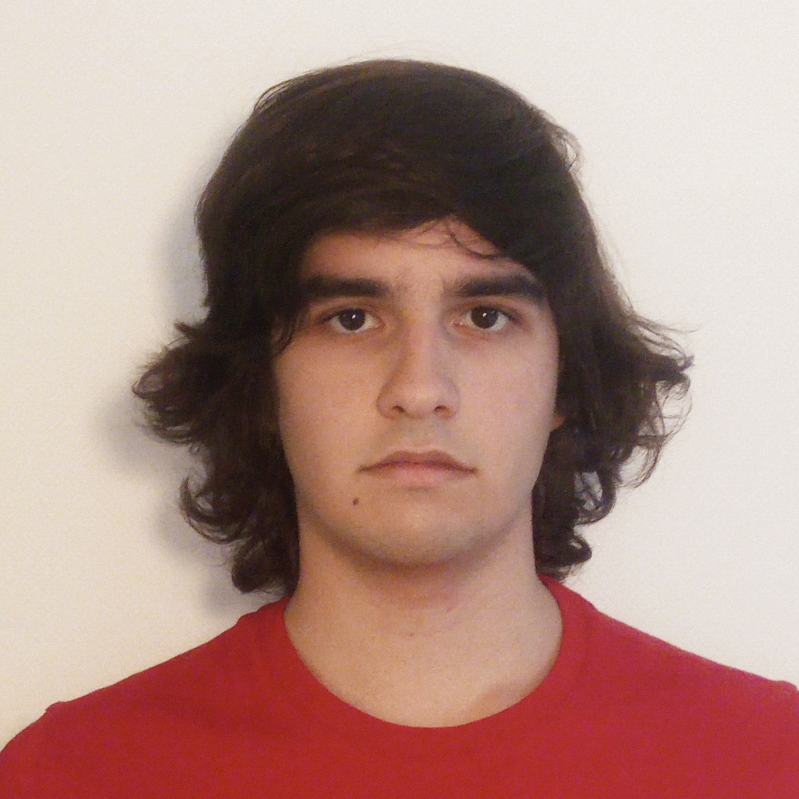
\includegraphics[width=3.5cm]{res/cover/A104348.png} &
            
\includegraphics[width=3.5cm]{res/cover/A90817.png} &
            
\includegraphics[width=3.5cm]{res/cover/A104179.png} \\

            Ana Oliveira & Humberto Gomes & Mariana Cristino & Sara Lopes \\
            A104437      & A104348        & A90817           & A104179
        \end{tabular}
    \end{center}
\end{adjustwidth}

\pagebreak

\begin{abstract}
    \textbf{\color{red} TODO - resumo}
\end{abstract}

\section{\emph{Generator}}

\textbf{\color{red} TODO - \emph{generator}}

\section{\emph{Engine}}

\textbf{\color{red} TODO - \emph{engine}}

\subsection{Torus}

O processo de criação do modelo 3D de um torus é dividido em duas fases: a geração do conjunto de
pontos que o constitui e o seu agrupamento em faces triangulares. Esta divisão tem origem na
estrutura de um ficheiro \texttt{.3d}, que separa os vértices de um modelo das suas faces.

O primeiro passo para a geração da nuvem de pontos de um torus é a definição das suas dimensões,
com o raio maior $R$ e o raio menor $r$. Como o torus é gerado a partir de uma parametrização
trigonométrica, cada ponto pode ser representado pelas seguintes equações:

$$
x = (-R + r \cos \phi) \cos \theta,
\hspace{1cm}
y = r \sin \phi,
\hspace{1cm}
z = (-R + r \cos \phi) \sin \theta.
$$

Onde $\theta$ representa o ângulo responsável por percorrer a circunferência maior do torus,
controlando a posição do ponto ao longo do anel principal, e $\phi$ representa o ângulo que
percorre a circunferência menor, determinando a posição do ponto dentro da secção transversal do
tubo. Ambos os ângulos variam no intervalo $[0, 2\pi]$.

O ângulo $\theta$ define a rotação do ponto em torno do eixo central do torus, percorrendo o
círculo principal de raio $R$. Assim, ao variar $\theta$, o ponto desloca-se ao longo do anel do
torus, mantendo-se sempre na mesma posição relativa dentro do tubo.

Já o ângulo $\phi$ determina a posição do ponto dentro da secção transversal do tubo, que tem raio
$r$. Ao variar $\phi$, o ponto descreve um movimento circular dentro do tubo, movendo-se ao longo
da circunferência menor do torus. Enquanto $\theta$ define onde o ponto se encontra ao longo do
torus, $\phi$ determina como o ponto está posicionado dentro da secção circular do tubo.

Para gerar uma malha de pontos distribuída uniformemente no torus, dividem-se os ângulos em fatias
($slices$) e segmentos ($stacks$), utilizando:

$$
\theta_i = i \cdot \frac{2\pi}{slices}, \quad i \in \{0, 1, \ldots, slices-1\}
$$

$$
\phi_j = j \cdot \frac{2\pi}{stacks}, \quad j \in \{0, 1, \ldots, stacks-1\}
$$

Assim, o torus é gerado iterando sobre os valores inteiros possíveis de $i$ e $j$, incrementando
primeiro $j$ e só depois $i$, o que dá origem a uma nuvem de pontos.

Depois de gerados, os vértices são agrupados em triângulos que compõem a superfície do torus. Para
isso, considera-se um vértice de referência, como $P_1$, juntamente com o vértice adjacente na
mesma fatia ($P_2$) e os dois vértices correspondentes na fila seguinte da grelha ($P_3$ e $P_4$).
Este processo repete-se para todos os vértices aplicáveis, garantindo que cada célula quadrangular
seja subdividida em dois triângulos. A figura seguinte ilustra esse processo, mostrando a estrutura
da malha e a organização dos triângulos resultantes.

\begin{figure}[H]
    \centering
    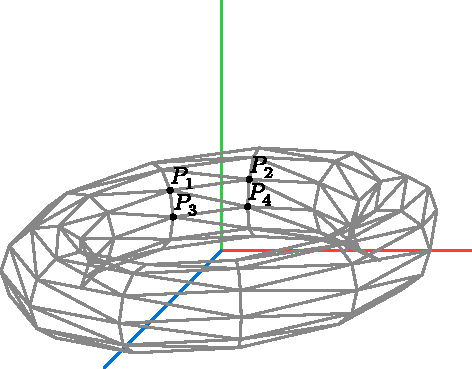
\includegraphics[width=0.4\textwidth]{res/figures/TorusTriangle.pdf}
    \caption{
        Triângulos de um torus gerado, mostrando a subdivisão da malha.
    }
\end{figure}

Uma otimização feita pela \emph{engine} é \emph{face culling}, ou seja, desenhar apenas as faces
voltadas para a câmara. No caso do torus, deseja-se que os seus triângulos estejam voltados para
fora, pelo que os seus vértices devem estar ordenados na ordem contrária à dos ponteiros do
relógio. Para os quatro pontos apresentados acima, os triângulos gerados são os seguintes:

$$
T_1 = (P_1, P_2, P_4)
\hspace{1cm}
T_2 = (P_1, P_3, P_4).
$$

\subsubsection{Normais e a ilusão de visibilidade da parte interna}

O \emph{torus} é uma superfície fechada e convexa, o que significa que cada ponto da sua superfície
tem uma normal bem definida, apontando para fora. Como a superfície é suavemente curvada, as
normais da parte externa do \emph{torus} apontam para fora do modelo, enquanto as normais da parte
interna do seu buraco também apontam para fora, seguindo a continuidade da superfície.

Em um modelo 3D ideal, a parte interna do \emph{torus} não deveria ser visível quando observado de
fora, pois a própria geometria bloquearia essa visão. No entanto, devido à forma como as normais
são orientadas, pode ocorrer um efeito onde a parte interna parece visível. Esse fenómeno acontece,
porque as normais da parte interna podem continuar alinhadas com as normais externas, fazendo com
que a renderização não diferencie corretamente o interior e o exterior.

Na prática, este problema pode ser mitigado através da aplicação de técnicas de
\emph{back-face culling}, que eliminam automaticamente as faces voltadas para longe da câmara,
garantindo que apenas a parte visível do modelo seja desenhada. Outra abordagem seria modificar o
material da superfície interna para diferenciar a iluminação, tornando a parte interna menos
visível quando renderizada.

\section{Resultados obtidos}

\textbf{\color{red} TODO - resultados}

\section{Conclusão e Trabalho Futuro}

\textbf{\color{red} TODO - conclusão}

\begingroup
\section{Bibliografia}
\renewcommand{\section}[2]{}

\begin{thebibliography}{9}
    \bibitem{exemplo}
        \href{https://youtu.be/dQw4w9WgXcQ}{Um item de exemplo na bibliografia}
\end{thebibliography}
\endgroup

\end{document}
